\documentclass[12pt]{article}
\usepackage{listings}
\usepackage{graphicx}
\usepackage{xcolor}

\begin{document}
\title{ECEC 471 Lab 2}
\author{Nicholas Sica}
\date{October 13, 2020}
\maketitle

\section{Introduction}
\subsection{Overview}
This lab is meant to guide us through the tools while designing an inverter as well as using the built-in analysis tools to decide on the best width to get a symmetric inverter.
CMOS circuits are designed by tying the outputs of a pull down and pull up network together. The pull up network in this lab is a singular pmos tied to voltage high, or Vdd, and
the pull down network is an nmos tied to voltage low, or ground. An inverter takes whatever signal it is given and flips it, causing a one to become a zero and a zero to become a one.
Rise time and fall time are the time it takes for the ouput to rise from 10\% to 90\% of the total voltage or fall from 90\% to 10\% of the total voltage.
Propagation delay is the time it takes for the output to appear after the input, usually measured by taking the difference of the 50\% marks of the input and output.
\subsection{Symmetric Inverters}
A symmetric inverter is an inverter whose rise and fall times are the same. In other words, the input and output voltage cross the half point of Vdd at the same time. We get a
symmetric inverter by keeping one of the transistor widths constant and changing the other.
\section{Simulation and Analysis}
\subsection{Schematic Design}
Figure~\ref{fig:asymm_schem} shows the transistor-level schematic of the inverter before the ideal width for the pmos was found. The initial width of both transistors was 90nm and
the length of both transistors is 50nm.
\begin{figure}[!htb]
  \centering
  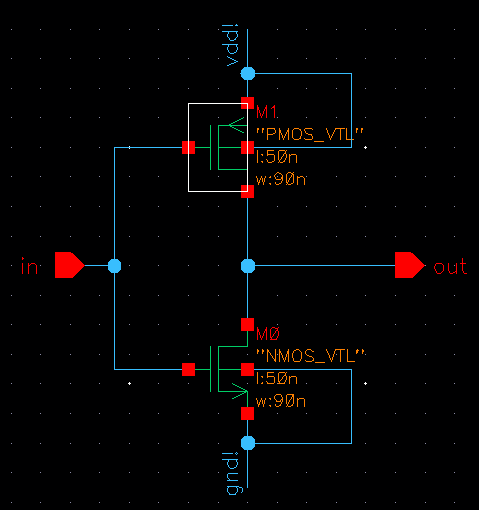
\includegraphics[width=4in]{figures/asymmetric_schematic.png}
  \caption{Transistor-level Non-symmetric Inverter Schematic}\label{fig:asymm_schem}
\end{figure}
Figure~\ref{fig:sim_schem} shows the simulation schematic with the source and load. A pulse is used so we can measure the rise and fall times as well as the propagation delay. The
pulse has an amplitude of 1.2V, a period of 100ns, a rise time of 10ps, 1 fall time of 10ps and a pulse width of 50ns. A 5fF capacitor was tied to the output to get it closer to a
realistic model where the inverter would have some capacitance.
\begin{figure}[!htb]
  \centering
  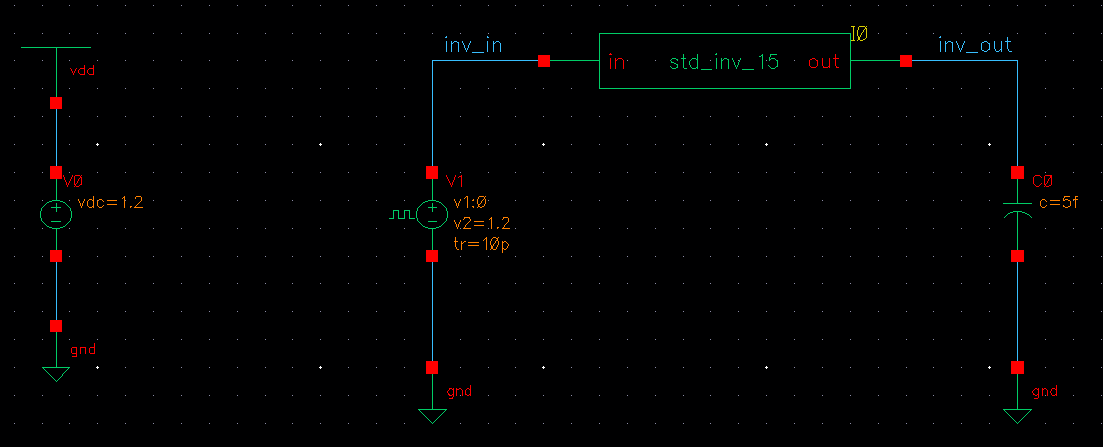
\includegraphics[width=5in]{figures/sim_schematic.png}
  \caption{Simulation Schematic}\label{fig:sim_schem}
\end{figure}
The transient analysis and DC response of the circuit are shown in Figure~\ref{fig:transient} and Figure~\ref{fig:asymm_dc} respectively. Using the transient analysis graphs a
rise time of 29.94ps, a fall time of 51.82ps, and propragation delay of 25.68ps were all easily found. The switching voltage was found to be 538.739mV using the DC response graph
which is not the desired 0.6V we want for a symmetric inverter.
\begin{figure}[!htb]
  \centering
  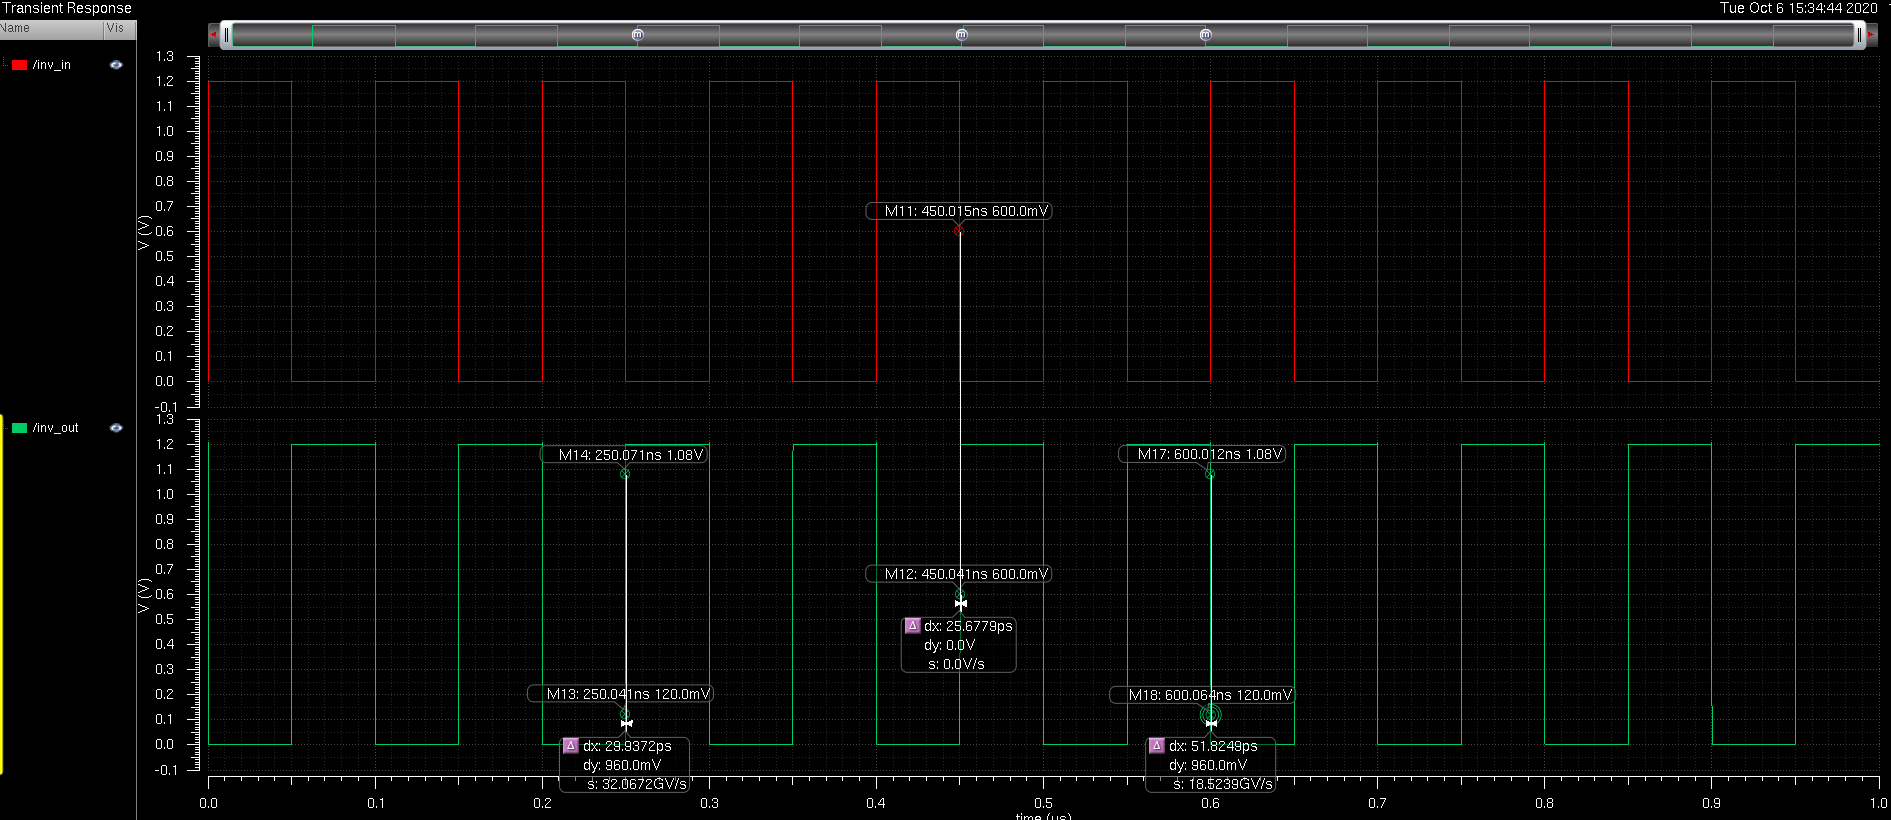
\includegraphics[width=5in]{figures/transient.png}
  \caption{Transient Analysis}\label{fig:transient}
\end{figure}
\begin{figure}[!htb]
  \centering
  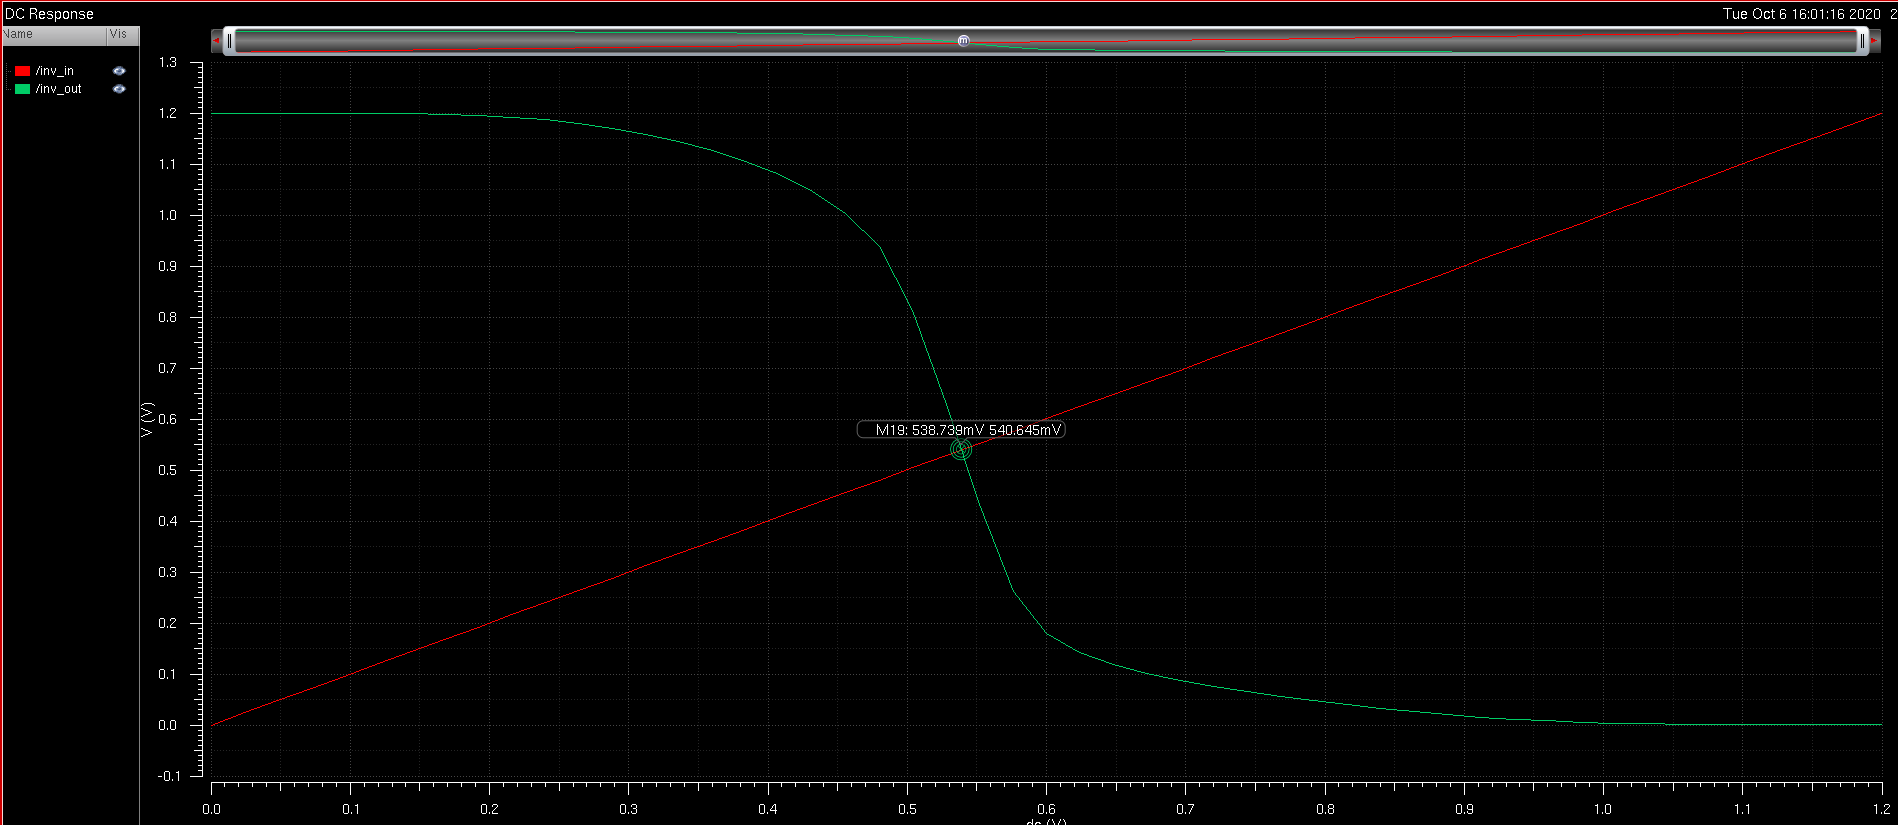
\includegraphics[width=5in]{figures/asymmetric_dc.png}
  \caption{DC Response of an Asymmetric Inverter}\label{fig:asymm_dc}
\end{figure}
To find the desired width of the pmos transistor, we used parametric analysis to get Figure~\ref{fig:parametric} and found that a width of 142.9412nm gave us a switching voltage of about 0.6V.
\begin{figure}[!htb]
  \centering
  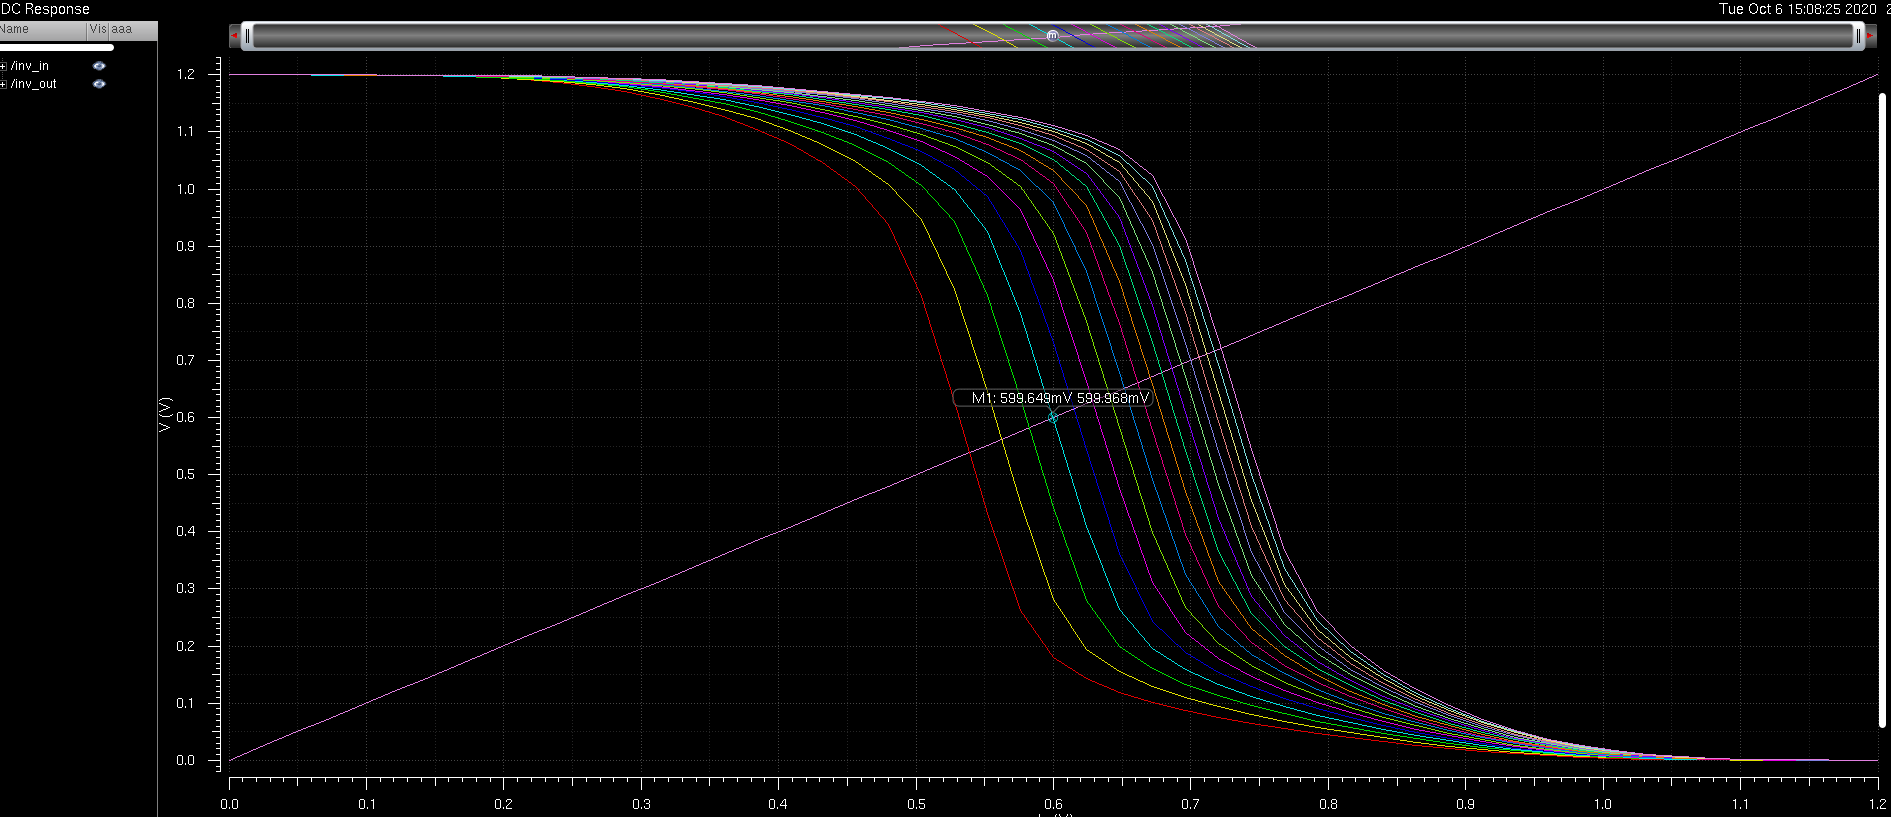
\includegraphics[width=5in]{figures/parametric.png}
  \caption{Parametric Analysis}\label{fig:parametric}
\end{figure}
The schematic was updated to use the new width in Figure~\ref{fig:sym_schem} and DC response was simulated and graphed again to give us Figure~\ref{fig:sym_dc} which shows a switching voltage of about 0.6V.
\begin{figure}[!htb]
  \centering
  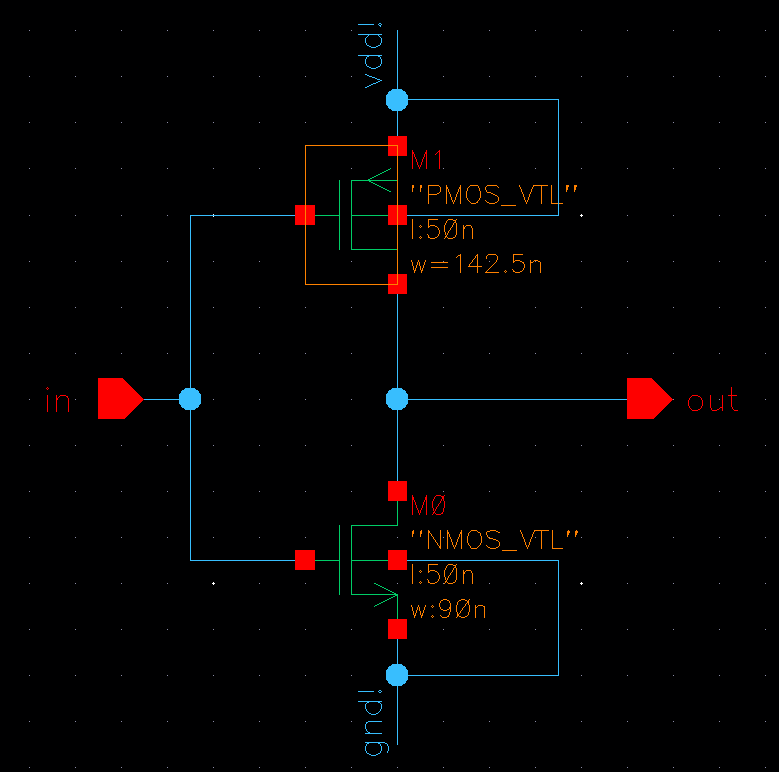
\includegraphics[width=4in]{figures/schematic.png}
  \caption{Symmetric Inverter Schematic}\label{fig:sym_schem}
\end{figure}
\begin{figure}[!htb]
  \centering
  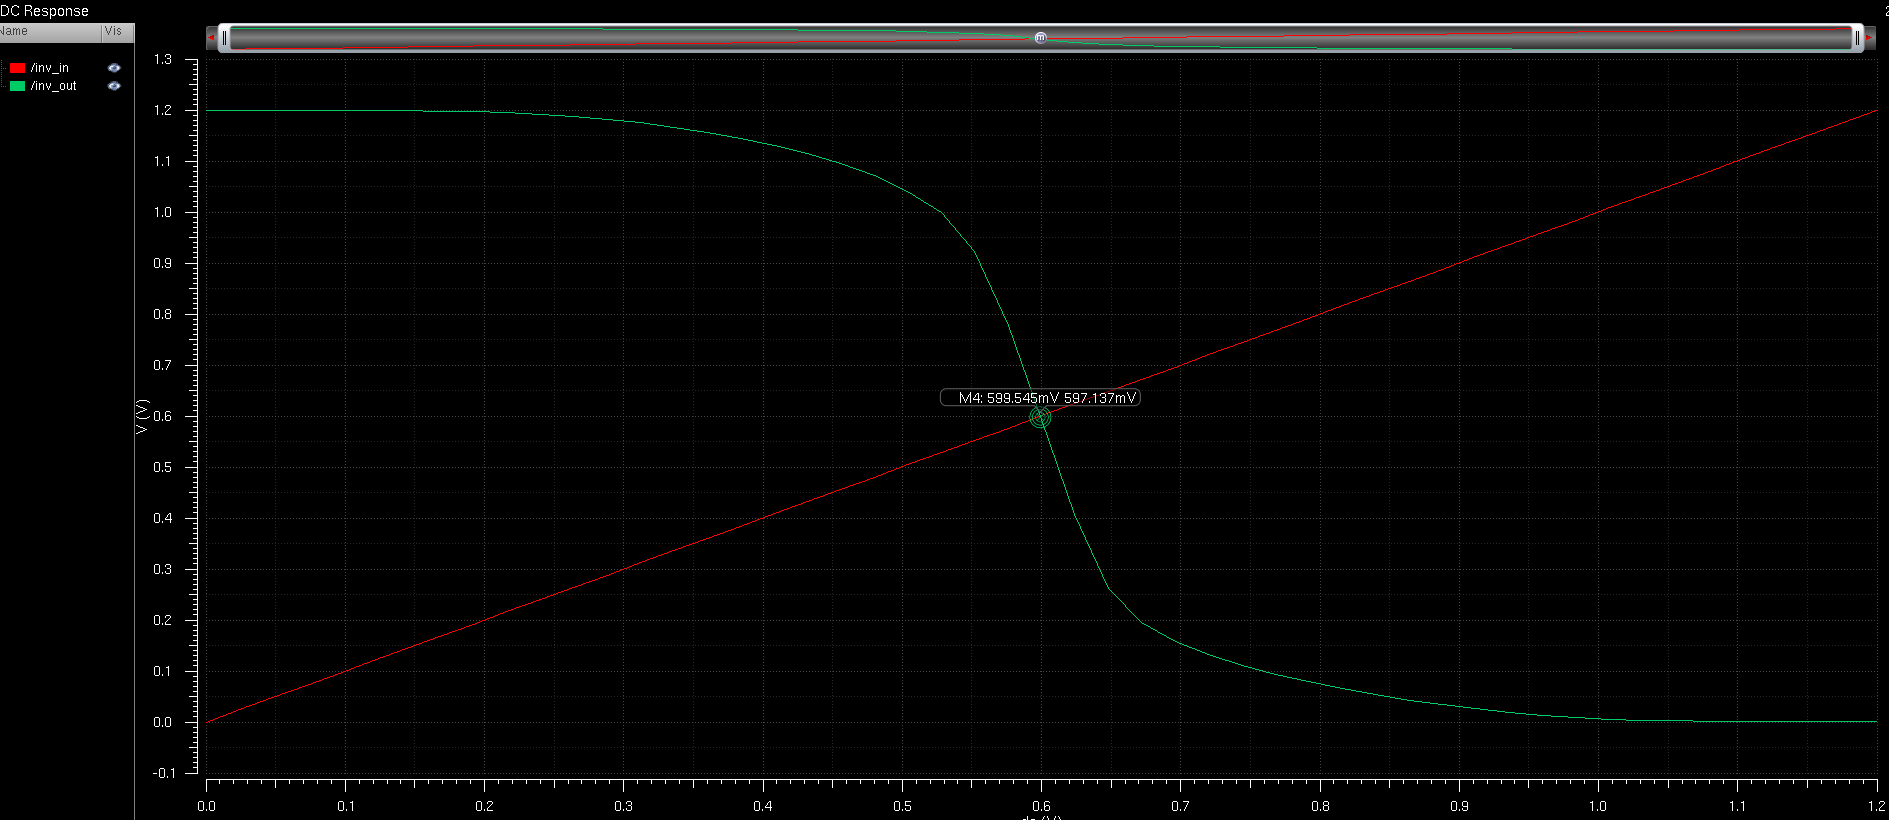
\includegraphics[width=5in]{figures/symmetric_dc.png}
  \caption{DC Response of a Symmetric Inverter}\label{fig:sym_dc}
\end{figure}
\subsection{Layout Design}
After the schematic was finished with it designed to be a symmetric inverter, layout was done. The pmos and nmos were built first, taking special care to make sure the width of the transistors match the schematic. The pmos and nmos are shown in Figure~\ref{fig:pmos} and Figure~\ref{fig:nmos} respectively. Afterwards, the Vdd and ground rails were added to the design as shown in Figure~\ref{fig:inverter_layout}.
\begin{figure}[!htb]
  \centering
  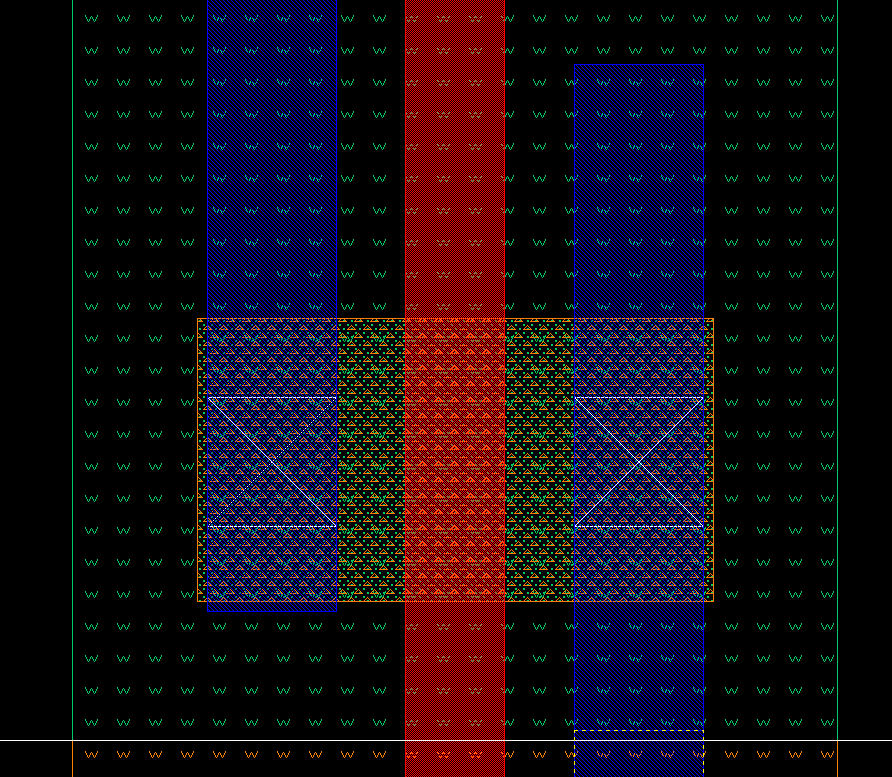
\includegraphics[width=4in]{figures/pmos.png}
  \caption{pMOS Layout}\label{fig:pmos}
\end{figure}
\begin{figure}[!htb]
  \centering
  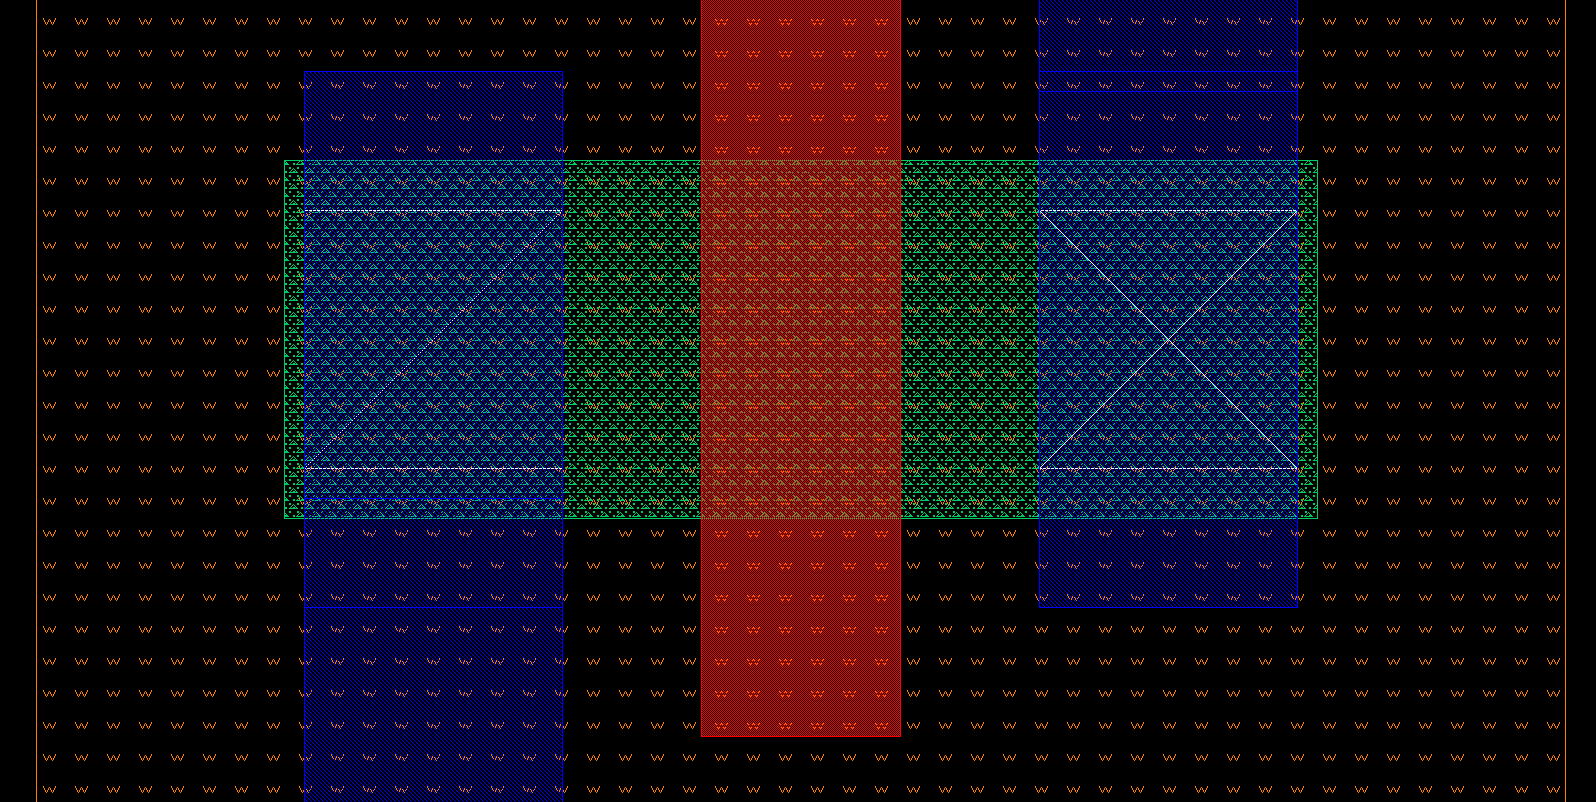
\includegraphics[width=4in]{figures/nmos.png}
  \caption{nMOS Layout}\label{fig:nmos}
\end{figure}
\begin{figure}[!htb]
  \centering
  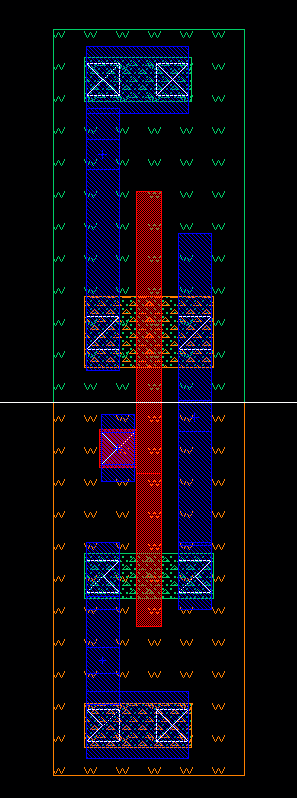
\includegraphics[width=2in,angle=90]{figures/layout.png}
  \caption{Inverter Layout}\label{fig:inverter_layout}
\end{figure}
Lastly, design rule checking(DRC) is used to make sure that no design rules are being violated and everything is fixed very painstakingly. The results can be seen in Figure~\ref{fig:drc}  After that layout versus schematic(LVS) was used to make sure our layout matches the design we modeled with the schematic and can be seen in Figure~\ref{fig:lvs}.
\begin{figure}[!htb]
  \centering
  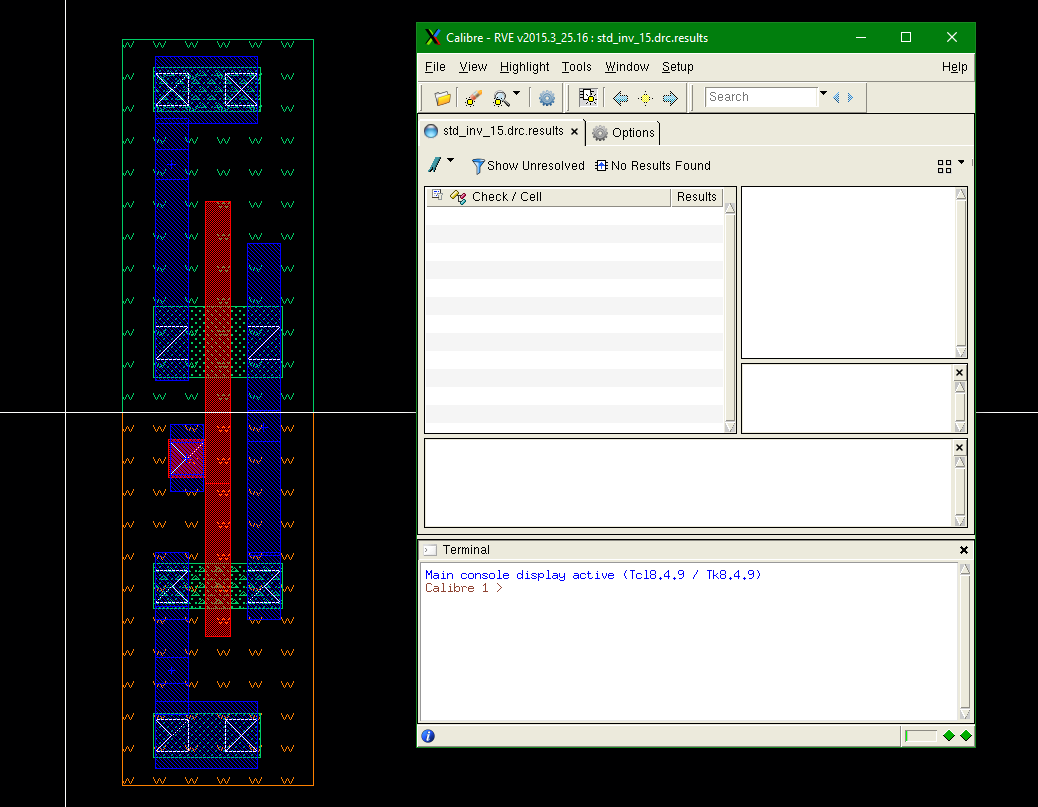
\includegraphics[width=5in]{figures/drc.png}
  \caption{DRC Results}\label{fig:drc}
\end{figure}
\begin{figure}[!htb]
  \centering
  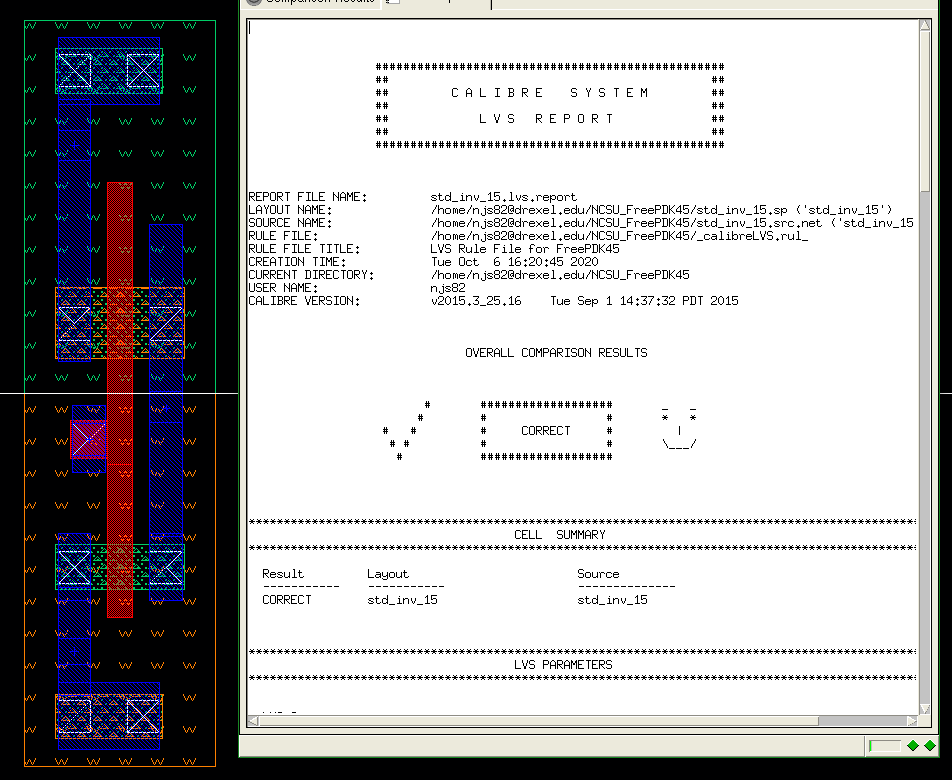
\includegraphics[width=5in]{figures/lvs.png}
  \caption{LVS Results}\label{fig:lvs}
\end{figure}
\section{Conclusion}
The lab was a very good way to work through building a schematic and deriving a layout from that schematic. It helped me get used to the tools and use them extensively to fine tune
my design and make sure everything was working as it should. It also helped me get a deeper understanding of the underlying technologies. The only thing I wish I could change is
making it easier to find the correct value for a symmetric inverter. Right now, it is a lot of try, check, and revise to get the perfect value.
\end{document}
%%% Local Variables:
%%% mode: latex
%%% TeX-master: t
%%% End:
